\clearpage
\begin{flushright}
	\textit{Лекция №7}
	\textit{2015.09.29}
\end{flushright}

Память, как ресурс, характеризуется памятью. Для общности: регистры процессора – как сверхбыстрая память. В кристалле процессора есть кэши. Они содержат актуальную информацию, ту, к которой в последнее время обращался. Затем оперативная память. В силу технологии производства, на порядок отстает в быстродействии. Процессор с памятью связаны локальной шиной. Все делается под управлением тактовых импульсов. Обращении к памяти – медленное действие большого количества тактов. Обращение к памяти получило название – цикл обращения к памяти. Затем внешняя память. Винчестер позволяет реализовывать виртуальную память. Дисковое пространство винчестера используется для организации виртуальной памяти. Связано с процессором соответствующей шиной. Винчестер – механическое устройство, соответственно оно медленнее. Иерархия памяти рассматривается с точки зрения близости к процессору. Флэш память подключается к usb портам, там нет механики. 

Вертикальное управление – передача информации с уровня на уровень. Сложная задача, реализуется через управление устройствами.

Одиночное ?? распределение характерно для древних систем. Возникает задача защиты, ОС от программы.

Современные компы – распараллеливание функций.

Мультипроцессные ОС – когда в памяти одновременно большое количество программ.

\section{Управлять памятью}, чтобы выделять память. Нужно иметь инфу о занятых разделах и свободных. Это можно осуществить с помощью двух таблиц. 

\begin{table}[H]
\caption{ТВР (таблица выделенных размеров)}
\begin{tabular}{|l|l|l|l|}
Номер раздела & Размер & Адрес & Состояние \\
\hline
1 & 8к & 312к & Распределен \\ 
\hline
2 & 32к & 320к & Распределен \\
\hline
3 & - & - & Пустой \\
\hline
4 & 120к & 384к & Распределен\\
\hline
\end{tabular}
\end{table}

\begin{table}[H]
\caption{ТСО (таблица свободных областей)}
\begin{tabular}{|l|l|l|l|}
Номер раздела & Размер & Адрес & Состояние \\
\hline
1 & 32к & 352к & Доступна \\ 
\hline
2 & 540к & 504к & Доступна \\
\hline
3 & - & - & Пустой эл \\
\hline
4 & - & - & Пустой эл\\
\hline
\end{tabular}
\end{table}

\section{Отредактировать таблицы}. 

Любое изменение распределения памяти отображается в соответствующих таблицах. 

\begin{figure}[H]
    \centering
    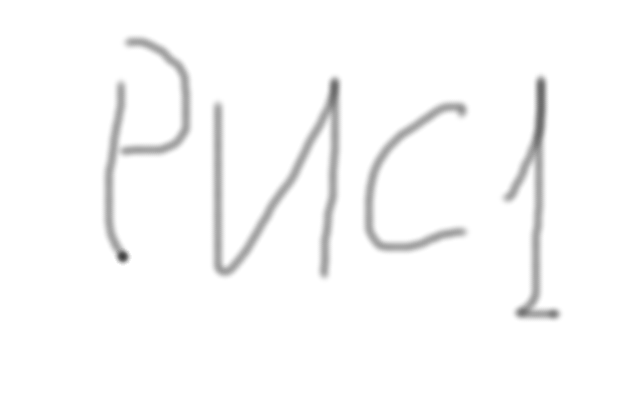
\includegraphics[width=\textwidth]{pic/1.png}
    \caption{Алгоритм объединения участков при освобождения памяти}
\end{figure}

Если мы постоянно загружаем и выгружаем программы, даже при наличии усилий по объединению соседних участков, в результате мы получим фрагментированную память. До 30\% памяти может съесть фрагментация.

\section{Стратегия выделения памяти}
\begin{enumerate}
    \item первый подходящий по размеру
    \item самый узкий 
    \item самый широкий. После загрузки программы у нас останется достаточно пространства, чтобы загрузить еще какую-то программу.
\end{enumerate} 

Как только отсортируем, используем продвинутые методы поиска.

\section{Перемещаемые разделы}

Если мы хотим перемещать программу в памяти, то нужно ввести логические адреса. Любая программа считает, что она начинается с нулевого адреса. В программе находятся смещения.

\begin{figure}[H]
    \centering
    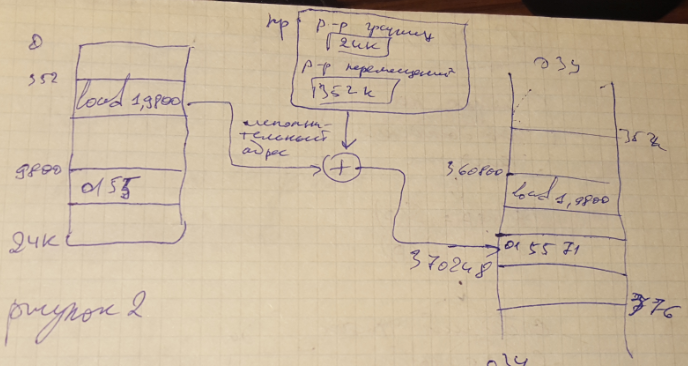
\includegraphics[width=\textwidth]{pic/2.png}
    \caption{pic}
\end{figure}

Мы рассмотрели, когда память выделяется программе целиком в последовательные адреса. Такое распределение в памяти называется связным, когда мы выделяем программе раздел последовательных адресов. Несвязное распределение памяти (либо страницами, либо сегментами). Так мы переходим к виртуальной памяти.

\section{Виртуальная память}
(кажущаяся, возможная)

Существует три схемы управления виртуальной памятью:
\begin{enumerate}
    \item управление памятью страницами по запросам;
    \item управление памятью сегментами по запросам;
    \item управление памятью сегментами, деленные на страницы по запросам.
\end{enumerate} 

По запросам – загрузка в память осуществляется по запросу. Запрос возникает, когда программа обращается к команде или данным, отсутствующей в памяти. 

Процесс начинает выполняться и в результате выполнения обращается к команде, отсутствующей в памяти, возникает страничное прерывание. Система загрузит эту страницу в память. А где же она? Дисковое адресное пространство в системах общего назначения делится на 2 части. Большая часть отведена для хранения файлов и управляется файловой системой. Меньшая часть отведена для свопинга (область свопинга (пейджинга) в зависимости от того, с чем мы работаем сегменты(страницы)). Виртуальную память можно представить, как пролонгированную на адресное пространство диска. В результате формируется виртуальное адресное пространство процесса. Каждый процесс, когда он создается, для него создается виртуальное адресное пространство. Это адресное пространство в системе описывается соответствующими таблицами. В Unix называются картами трансляции адресов (страницы сегментов или страниц).

\subsection{Управление памятью страницами по запросам}

Адресное пространство процесса делится на страницы.

\begin{figure}[H]
    \centering
    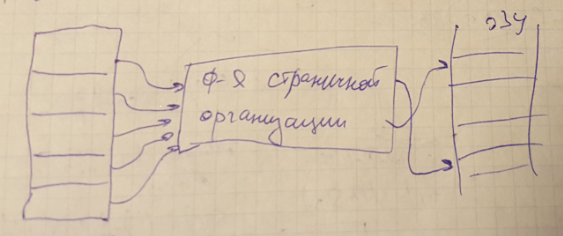
\includegraphics[width=\textwidth]{pic/3.png}
    \caption{pic}
\end{figure}

Страница – на которую делится адресное пространство процесса. А страницу, на которую делится физическая память называют фреймов.

\subsubsection{Прямое отображение}
Отображаем страницы виртуального пространства на физическую. В процессоре имеется регистр, в который загружается начальный адрес таблицы страниц.

\begin{figure}[H]
    \centering
    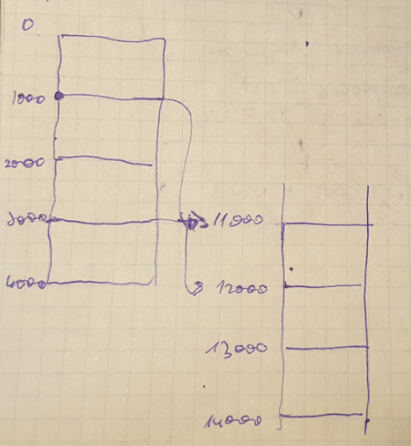
\includegraphics[width=\textwidth]{pic/4.png}
    \caption{pic}
\end{figure}

\begin{figure}[H]
    \centering
    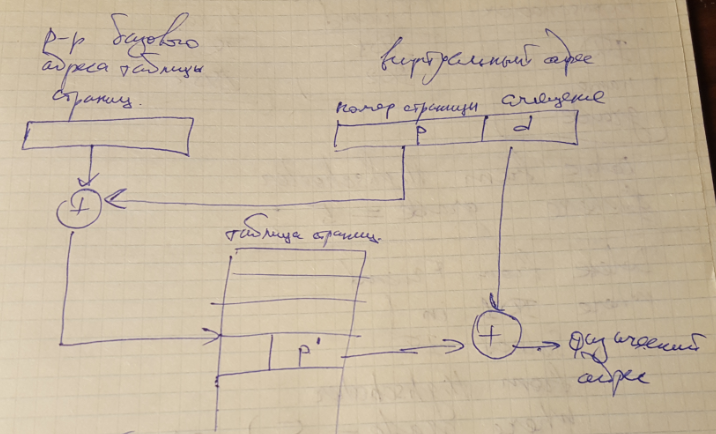
\includegraphics[width=\textwidth]{pic/5.png}
    \caption{pic}
\end{figure}

Таблица страниц находится в оперативной памяти. Таких страниц столько – сколько процессов. Если в системе большое количество процессов, каждый процесс имеет большое адресное пространство, таблица страниц так же занимает много памяти, если в данный момент этот процесс находиться в состоянии блокировки, или sleep, то нет смысла эту таблицу держать в памяти. Каждую команду будет обращение к таблице. Увеличивается мультипроцессность. 